\chapter{Auswertung}
\label{kap:auswertung}

\section{Metriken und Bewertungsprotokoll}
\label{sec:metriken}

Eine Detektion gilt als Treffer, wenn ihre Box eine Ground-Truth-Box mit einer
\emph{Intersection over Union} von mindestens $t$ überdeckt; jede
Ground-Truth-Box kann höchstens einmal getroffen werden. Daraus folgen
\emph{Precision} $P$, \emph{Recall} $R$ und deren harmonisches Mittel $F_1$;
berichtet wird stets das beste $F_1$ über alle Konfidenzschwellen samt der
zugehörigen Schwelle $c^*$ -- der Betriebspunkt, den man in einer Anwendung
wählen würde. \emph{mAP} ist die Fläche unter der Precision-Recall-Kurve
\parencite{everingham2010}; \mAPfifty{} verwendet $t = 0{,}5$, \mAPseven{}
$t = 0{,}75$ und \mAPall{} den Mittelwert über $t = 0{,}50; \dots; 0{,}95$ nach
COCO-Konvention \parencite{lin2014coco}. Leitgröße dieser Arbeit ist
\mAPfifty{}: Bei Objektdurchmessern um 20\px{} misst \mAPall{} zu einem
erheblichen Teil die Pixelauflösung und die Labelkonvention und nicht die
Detektionsgüte -- Abschnitt~\ref{sec:boxversatz} weist das nach.

Die Bewertung erfolgt über eine eigene Implementierung, weil die mittlere
Treffer-IoU und der $F_1$-optimale Betriebspunkt gebraucht werden -- Größen, die
die Standardfunktion der Werkzeugkette nicht ausgibt. Zur Absicherung wurde sie
gegen die Referenzimplementierung geprüft: \code{val} 0,886/0,597 gegen
0,897/0,599 und \code{test} 0,956/0,466 gegen 0,949/0,451
(\mAPfifty{}/\mAPall{}); die Abweichung von maximal 1,5\PP{} ist durch
Detailunterschiede in der AP-Interpolation erklärbar.

\section{Hauptergebnis und Sim-to-Real-Abstand}
\label{sec:hauptergebnis}

\begin{table}[htbp]
\centering
\caption[Hauptergebnis]{Ergebnis des besten Modells bei nativem Maßstab.
$c^*$ ist die $F_1$-optimale Konfidenzschwelle, $P$ und $R$ sind Precision und
Rückruf an diesem Betriebspunkt.}
\label{tab:hauptergebnis}
\footnotesize
\begin{tabular}{@{}lrrrrrrr@{}}
\toprule
\textbf{Split} & \mAPfifty{} & \mAPseven{} & \mAPall{} & \textbf{bestes $F_1$} &
$c^*$ & $P$\,/\,$R$ & \textbf{mittl.\ IoU} \\
\midrule
\code{val} (real)  & \textbf{0,886} & 0,793 & 0,597 & 0,862 & 0,336 & 0,872\,/\,0,852 & 0,824 \\
\code{test} (real) & \textbf{0,956} & 0,326 & 0,466 & 0,971 & 0,263 & 1,000\,/\,0,944 & 0,746 \\
\code{sval} (synth.) & 0,982 & 0,935 & 0,828 & 0,964 & 0,450 & 0,972\,/\,0,956 & 0,899 \\
\bottomrule
\end{tabular}
\end{table}

Ein ausschließlich auf synthetischen Bildern trainiertes Modell erreicht auf
echten, nie im Training gesehenen Aufnahmen \mAPfifty{} von \textbf{0,886} und
\textbf{0,956} -- die Antwort auf die Aufgabenstellung. Am $F_1$-optimalen
Betriebspunkt findet es 85\,\% (\code{val}) bzw.\ 94\,\% (\code{test}) der
Objekte; auf \code{test} sitzt dabei \emph{jede} Detektion auf einem annotierten
Objekt (Precision 1,000). Bei der auf \code{val} gewählten Inferenzauflösung
bleibt \mAPfifty{} auf \code{test} bei 0,956, mit Test-Time-Augmentation steigt
es auf 0,963.

Der auffällige Unterschied zwischen den Splits -- \mAPseven{} 0,793 auf
\code{val}, aber nur 0,326 auf \code{test} bei höherem
\mAPfifty{} -- ist kein Widerspruch. Ein Teil davon ist die in
Abschnitt~\ref{sec:ioukleinobjekt} beschriebene Empfindlichkeit der IoU bei
kleinen Objekten: Die Objekte in \code{test} sind kleiner (Median 17,0 gegen
27,4\px), und die mittlere Treffer-IoU bestätigt den Unterschied direkt (0,746
gegen 0,824). Der größere Teil ist ein \emph{systematischer Größenversatz
zwischen Generatorlabel und Handannotation}, der in
Abschnitt~\ref{sec:boxversatz} aufgeschlüsselt wird. \mAPall{} ist bei dieser
Objektgröße daher weniger ein Maß für die Detektionsqualität als für
Pixelauflösung und Labelkonvention -- eine Feststellung, die für alle folgenden
Tabellen gilt. Ein Qualitativbild der Detektionen zeigt
Abbildung~\ref{abb:qualitativ} im Anhang.


\absatz{Sim-to-Real-Abstand.}\label{sec:simtoreal}
Der Split \code{sval} besteht aus 400 synthetischen Bildern derselben Pipeline
mit anderem Seed und trennt damit zwei Fragen: \emph{Kann das Modell die Aufgabe
überhaupt?} und \emph{überträgt es sich auf echte Bilder?} Der Abstand beträgt
$0{,}982 - 0{,}886/0{,}956 = \mathbf{9{,}6}$ bzw.\ $\mathbf{2{,}6}$\PP{}
\mAPfifty{}; bei \mAPall{} sind es 23,1 (\code{val}) bzw.\ 36,2 (\code{test})
Prozentpunkte. Er ist damit \textbf{klein} -- auf \code{test} sehr klein -- und
\textbf{weit entfernt von dem Muster, das reines Artefaktlernen erzeugen
würde}: Wäre die Pipeline an
einer der Signaturen S1--S6 durchlässig, so wäre \code{sval} nahezu perfekt
($>0{,}99$) und die realen Bilder katastrophal. Genau dieses Muster tritt nicht auf -- der einzige
\emph{direkte} empirische Hinweis darauf, dass die Anti-Abkürzungs-Maßnahmen
greifen, und ein Indiz, kein Beweis.

\absatz{Die Schranke, mit Werten besetzt.} Gleichung~\eqref{eq:bendavid} lässt
sich mit diesen Zahlen teilweise füllen. Als Platzhalter für den Fehlerterm dient
$\varepsilon = 1 - \mAPfifty{}$ -- die Schranke ist für den
0-1-Klassifikationsfehler formuliert, die Rechnung zeigt daher die
\emph{Struktur} und ist kein Beweis. Mit $\varepsilon_S = 1 - 0{,}982 = 0{,}018$
auf \code{sval} und $\varepsilon_T = 1 - 0{,}956 = 0{,}044$ auf \code{test} folgt
aus Gleichung~\eqref{eq:bendavid-diff}
\[
d_{\mathcal{H}\Delta\mathcal{H}} + \lambda \;\geq\; 0{,}044 - 0{,}018
\;=\; 0{,}026 .
\]
Der Größenversatz aus Abschnitt~\ref{sec:boxversatz} trägt dazu \emph{nichts}
bei: Eine abweichende Labeldefinition wäre genau ein $\lambda$-Beitrag, aber die
Sensitivitätsrechnung zeigt, dass ein Angleichen der Boxgröße \mAPfifty{} nicht
verbessert, sondern leicht senkt (Tabelle~\ref{tab:boxsens} im Anhang). Bei der
Zuordnungsschwelle 0,5 ist die Konventionsdifferenz also wirkungslos, und die
verbleibenden 2,6\PP{} sind im Wesentlichen Verteilungsdivergenz -- klein, aber
nicht wegerklärbar.

Die Gegenprobe macht die Größenordnung deutlich. Hätte das Netz statt der
Rohrenden die Einfügeartefakte gelernt, so wäre \code{sval} nahezu perfekt
($\varepsilon_S \approx 0{,}005$) und die realen Bilder katastrophal
($\varepsilon_T \approx 0{,}95$); die Schranke ergäbe dann
$d + \lambda \geq 0{,}94$ -- den \emph{36-fachen} Wert. Dass stattdessen 0,026
gemessen werden, ist die formale Fassung des Arguments oben und zeigt zugleich
seine Grenze: Die Ungleichung schließt eine große Divergenz nicht \emph{aus}, sie zeigt
nur, dass die Daten sie nicht erzwingen. Genau deshalb bleibt es ein Indiz.

\section{Die Inferenzauflösung}
\label{sec:imgsz}

Die Inferenzauflösung ist der einzige Parameter, der nach dem Training noch frei
ist, und deshalb der einzige, dessen Wert gemessen statt begründet wird. Ein
eigenes Experiment ist das nicht -- es wird kein Modell neu trainiert, sondern
dasselbe Modell bei zehn Auflösungen ausgewertet. Gemustert werden neun Stufen zwischen 640 und 2464\px{} sowie
der native Maßstab, gemessen auf der \code{yolo11s}-Baseline. Ausgewählt wird
die Stufe mit dem höchsten \mAPall{} auf \code{val}, und zwar ausschließlich
dort; der so gefundene Wert wird unverändert auf beide Splits angewandt -- eine
Wahl je Split wäre eine Hyperparameterselektion auf dem Testsatz und würde
dessen Zahlen wertlos machen. Das Kriterium ist bewusst \mAPall{} und nicht
\mAPfifty{}, weil es die Lokalisierungsgüte mitbewertet; es stand vor den Läufen
fest und gilt unverändert für alle in dieser Arbeit ausgewerteten Modelle. Für
die Baseline fallen beide Metriken auf \code{val} auseinander: \mAPfifty{} ist
bei 1600 am höchsten, \mAPall{} bei 1920 (Tabelle~\ref{tab:imgszvoll} im
Anhang); gewählt wurde daher 1920.

\begin{table}[htbp]
\centering
\caption[Sweep der Inferenzauflösung]{Auszug aus dem Sweep der
Inferenzauflösung. Nativer Maßstab ist 2464 (\code{val}) bzw.\ 1600
(\code{test}); der vollständige Sweep umfasst neun Stufen je Split.}
\label{tab:imgsz}
\footnotesize
\begin{tabular}{@{}lrrrrr@{}}
\toprule
\code{imgsz} & \code{val} \mAPfifty{} & \code{val} $R$ &
\code{test} \mAPfifty{} & \code{test} $R$ & \code{val} pred/gt \\
\midrule
640  & 0,435 & 0,398 & 0,512 & 0,449 & 50/88 \\
960  & 0,852 & 0,773 & 0,881 & 0,809 & 74/88 \\
1280 & 0,887 & 0,841 & 0,917 & 0,865 & 84/88 \\
1600 & \textbf{0,904} & 0,898 & \textbf{0,956} & 0,944 & 98/88 \\
1920 & 0,893 & 0,909 & \textbf{0,956} & 0,921 & 100/88 \\
2464 & 0,886 & 0,852 & 0,941 & 0,899 & 86/88 \\
\bottomrule
\end{tabular}
\end{table}

Von \code{imgsz}~640 auf 1600 steigt \mAPfifty{} auf \code{val} von 0,435 auf
0,904 -- eine Verdopplung und mit 47\PP{} der größte gemessene Einzeleffekt der
Arbeit, größer als jede einzelne Entscheidung in der Augmentierungspipeline. Die
Erklärung ist rein geometrisch und wurde in
Abschnitt~\ref{sec:ioukleinobjekt} vorhergesagt: Bei \code{imgsz}~640 wird das
2459\px{} breite \code{val}-Bild um den Faktor 0,26 verkleinert, die Objekte
schrumpfen von 20--36 auf 5--9\px{} und unterschreiten die Schrittweite~8 der
feinsten Detektionsebene. Der Rückruf bricht entsprechend auf 0,398 ein: Das
Modell \emph{findet} die Objekte nicht mehr, es lokalisiert sie nicht bloß
schlechter.

Bemerkenswert ist, dass das Optimum \emph{nicht} am nativen Maßstab liegt --
allerdings nur auf \code{val}: Dort liegt das \mAPfifty{}-Maximum bei 1600 und
damit deutlich \emph{unter} dem nativen Maßstab von 2464 (0,904 gegen 0,886).
Auf \code{test} sind nativer Maßstab und 1920 dagegen praktisch gleichwertig
(0,956 gegen 0,956) -- dort ist über die Auflösung nichts zu gewinnen. Der Grund
für die Richtung des Effekts liegt in der Trainingsverteilung: Der Generator erzeugt
Objekte mit Median 22,5\px{}, \code{test} hat nur 17,0\px{} Median -- eine
leichte Hochskalierung schiebt die
Testobjekte in die Mitte der Trainingsverteilung. Daraus folgt die Empfehlung,
\emph{nicht} auf den nativen Maßstab zu skalieren, sondern so, dass die erwartete
Objektgröße im Netzeingang etwa dem Median der Trainingsverteilung entspricht --
hier rund 22\px. Der Objektgrößenbereich des Generators und die
Inferenzauflösung sind damit \emph{nicht} unabhängig voneinander wählbar. Die
übrigen Inferenzparameter sind dagegen unkritisch: Der NMS-Schwellwert bewegt zwischen
0,3 und 0,9 nur 3\PP{} (benachbarte Rohrenden haben mindestens 0,85 Durchmesser
Abstand, ihre Boxen überlappen also kaum), \code{max\_det} ist ab 100 gesättigt
(bei 50 dagegen katastrophal, weil die Ausgabe hart abgeschnitten wird und nur
50 der 88 Objekte erreicht), und FP16 liefert bitidentische
Ergebnisse. Test-Time-Augmentation bringt $+2{,}1$\PP{} auf \code{val} und
$+0{,}7$ auf \code{test} bei doppeltem Rechenaufwand \parencite{shanmugam2021} --
ohne Echtzeitanforderung lohnend.

\section{Das Experiment: Wie viel Verdeckung in den Trainingsdaten?}
\label{sec:ablation}

Dies ist das Experiment der Arbeit, und es ist bewusst dieses: Die
Okklusionserzeugung ist die
aufwendigste Einzelstufe der Pipeline -- sie erfordert die Okkluder-Bibliothek,
das Tiefenmodell und die exakte Sichtbarkeitsrechnung. Zahlt sich der Aufwand
messbar aus?

\absatz{Versuchsaufbau.} Drei Datensätze unterscheiden sich \emph{ausschließlich}
im Verdeckungsgrad; alles andere ist identisch (derselbe Seed, 3000 Bilder,
dieselben Hyperparameter, 30 Epochen). Arm~\textbf{A0} hat keine quer liegenden
Stangen, keine Fremdkörper und keinen Schaft, der vor einer Stirnfläche kreuzt;
\textbf{A1} ist die Baseline aus Kapitel~\ref{kap:pipeline}; \textbf{A2} hat in
jedem Bild Stangen, mehr Fremdkörper und mehr quer vor dem Stapel liegende Rohre.
Der Rohrschaft \emph{hinter} der Stirnfläche bleibt in allen Armen erhalten -- er
ist physikalische Randbedingung, keine Augmentierung. Die Kontrolle ist besser als
bei einer gewöhnlichen Datensatz-Ablation: Weil der Seed identisch ist, rendern
alle drei Arme \textbf{genau dieselben 86\,617 Instanzen an denselben
Positionen}. Der einzige Unterschied ist, wie viel davon verdeckt wird -- und als
Folge, wie viele Labels die Sichtbarkeitsregel verwirft.

\begin{table}[htbp]
\centering
\caption[Okklusionsablation]{Okklusionsablation: erzeugte Datensätze (links) und
Ergebnis bei nativem Maßstab (rechts). \textbf{Vier der fünf Metrikspalten}
sind über die drei Arme monoton; \mAPall{} auf \code{test} nicht -- dort liegt
A1 über A2.}
\label{tab:ablation}
\footnotesize
\begin{tabular}{@{}lrrr|rrrrr@{}}
\toprule
\textbf{Arm} & \textbf{Labels} & \textbf{Sichtb.} & \textbf{teilverd.} &
\code{val} \mAPfifty{} & \code{val} \mAPall{} &
\code{test} \mAPfifty{} & \code{test} \mAPall{} & \code{test} $F_1$ \\
\midrule
A0 ohne     & 82\,950 & 0,977 & 12,0\,\% & 0,888 & 0,606 & 0,9577 & 0,441 & 0,928 \\
A1 Baseline & 68\,281 & 0,902 & 29,9\,\% & 0,924 & 0,609 & 0,9584 & \textbf{0,482} & 0,949 \\
A2 stark    & 55\,833 & 0,852 & 40,7\,\% & \textbf{0,930} & \textbf{0,620} &
\textbf{0,9596} & 0,479 & \textbf{0,959} \\
\bottomrule
\end{tabular}
\end{table}

Drei Befunde. \emph{(1) Der Effekt ist überwiegend monoton:} Von A0 zu A2 steigen
auf \code{val} \mAPfifty{} um 4,2\PP{} und \mAPall{} um 1,4\PP{}, auf dem
unberührten Testbild das $F_1$ um 3,1\PP{} -- jeweils über alle drei Stufen in
derselben Richtung. Zwei Einschränkungen: \mAPfifty{} auf \code{test} ist mit
0,19\PP{} Spanne praktisch gesättigt (alle drei Arme liegen bei 0,96), und
\mAPall{} auf \code{test} verläuft nicht monoton -- A1 liegt dort über A2. \emph{(2) Der Gewinn entsteht gegen einen Verlust an Supervision:} A2
hat durch die stärkere Verdeckung \textbf{32,7\,\% weniger Labels} als A0
(55\,833 gegen 82\,950 bei identischer Bildzahl und identischen gerenderten
Instanzen). Der Okklusionsvorteil überkompensiert also einen deutlichen Verlust an
Trainingssignal -- der stärkste Einzelbeleg dafür, dass die Okklusionsstufe kein
Beiwerk ist: Wären die zusätzlichen Labels wertvoller als die zusätzliche
Schwierigkeit, müsste A0 gewinnen. \emph{(3) Ohne Verdeckung ist die Aufgabe zu
leicht:} A0 erreichte sein bestes Modell bereits in Epoche~3 und verbesserte sich
in den folgenden 20 Epochen nicht mehr, A1 und A2 verbesserten sich bis zur
letzten Epoche~30 durchgehend.

\absatz{Einordnung und Einschränkungen.} Der Befund ist mit den Ergebnissen zu
Cutout und Random Erasing verträglich
\parencite{devries2017cutout,zhong2020erasing}, geht aber über sie hinaus: Dort
wird Bildinhalt gelöscht und das Label beibehalten, hier verdeckt ein Objekt mit
eigener Textur, und das Label wird bei zu starker Verdeckung entfernt -- die
entstehenden Beispiele sind damit sowohl schwierigere Positive als auch korrekte
harte Negative. Drei Vorbehalte bleiben. Erstens liegt der Effekt
\emph{innerhalb} des Konfidenzintervalls von $\pm 0{,}05$ (\code{val}) bzw.\
$\pm 0{,}02$ (\code{test}); belastbar ist nicht die einzelne Differenz, sondern
die \emph{Konsistenz} -- dieselbe Richtung in vier von fünf Metrikspalten über
alle drei Stufen, was bei reinem Rauschen unwahrscheinlich wäre. Nicht monoton
verläuft \mAPseven{} auf \code{val} (0,812 / 0,760 / 0,775); die Aussage betrifft
das Finden der Objekte, nicht die Präzision der Boxen. Zweitens sind Labelzahl und
Okklusionsanteil nicht entkoppelt -- mehr Verdeckung heißt zwangsläufig mehr
verworfene Labels. Drittens waren A1 und A2 nach 30 Epochen nicht auskonvergiert;
die Aussage ist konservativ, aber nicht abgeschlossen.

% ===========================================================================
% Experiment 3 (P2-Detektionskopf) -- geparkt.  Begruendung: Die Arbeit
% behaelt genau ein Experiment, und zwar das einzige, das die eigene
% Pipeline prueft (Okklusionsablation).  Der P2-Vergleich ist eine
% Architekturfrage und kostet mit Abbildungen und Tabellen rund fuenf Seiten.
% ACHTUNG: Die test-Zahlen dieses Blocks sind gegen 86 statt der aktuellen 89
% Objekte gerechnet und damit veraltet.  Bei Reaktivierung muessen yolo26s und
% yolo26s-p2 auf test neu ausgewertet werden.
% Reaktivieren: \iffalse/\fi entfernen und die Verweise in
% 01, 02, 03, 06, 08 zuruecknehmen (siehe git-freie Kopie kapitel_kurz/).
% ===========================================================================
\iffalse

\section{Experiment 3: der P2-Detektionskopf}
\label{sec:p2}

\subsection{Frage und Versuchsaufbau}

Abschnitt~\ref{sec:ioukleinobjekt} hat die Auflösungsgrenze quantifiziert: Ein
Objekt mit Durchmesser $d$ belegt auf einer Ebene mit Schrittweite $S$ im Mittel
$\pi d^2/(4S^2)$ Gitterzellen, und unterhalb von $d < S\sqrt{2}$ existieren
Lagen, bei denen \emph{kein} Zellzentrum im Objekt liegt. Für die feinste
Standardebene P3 ($S = 8$) liegt diese Grenze bei 11,3\px{} -- genau im Bereich
der hier auftretenden Objektgrößen. Die Architekturseite bietet dafür eine
direkte Gegenmaßnahme: einen zusätzlichen Detektionskopf auf der Ebene P2 mit
Schrittweite~4 (Abbildung~\ref{abb:pyramide}). Dieses Experiment prüft, was er
bringt und was er kostet.

Verglichen werden \code{yolo26s} (Ebenen P3--P5) und \code{yolo26s-p2}
(Ebenen P2--P5). Bewusst \emph{nicht} verglichen wird mit der yolo11s-Baseline:
Ein Vergleich über Modellfamilien hinweg vermischte den Effekt der Kopfstruktur
mit dem der Familie. Beide Modelle werden auf demselben Datensatz, mit denselben
Hyperparametern und demselben Budget trainiert und mit demselben
Bewertungsframework gemessen; \code{yolo26s-p2} startet von den
\code{yolo26s}-Gewichten, damit auch die Initialisierung vergleichbar ist.

\subsection{Was der zusätzliche Kopf architektonisch bedeutet}

Der Unterschied liegt allein im Neck und im Kopf. Die
Standardkonfiguration führt den Aufwärtspfad des Feature-Pyramid-Netzwerks
\parencite{lin2017fpn} bis P3 und schickt von dort einen Abwärtspfad über P4 zu
P5; die \code{-p2}-Variante setzt den Aufwärtspfad um eine Stufe fort,
verknüpft ihn mit der P2-Karte des Backbones und startet den Abwärtspfad
entsprechend eine Ebene tiefer. Der Detektionskopf erhält damit vier statt drei
Eingänge. Weil die Eingangsbreite des Kopfes seine internen Kanalzahlen bestimmt
und der neue, feinste Eingang schmaler ist als der bisherige, hat die
\code{-p2}-Variante sogar \emph{weniger} Parameter als das Basismodell --
sie ist kein größeres, sondern ein \emph{feiner aufgelöstes} Netz.

\begin{table}[htbp]
\centering
\caption[Kennzahlen der beiden Varianten]{Kennzahlen der beiden Varianten. Die
Prädiktionspositionen und Gittergrößen gelten für eine Eingabe von
$1024\times1024$; GFLOPs und Parameter sind die Werte der tatsächlich
trainierten Modelle (eine Klasse), Speicher und Zeit die gemessenen Werte des
Trainingslaufs bei \code{imgsz}=1024 und Batch~16.}
\label{tab:p2kennzahlen}
\footnotesize
\begin{tabularx}{\textwidth}{@{}Xrr@{}}
\toprule
\textbf{Kenngröße} & \textbf{\code{yolo26s}} & \textbf{\code{yolo26s-p2}} \\
\midrule
Detektionsebenen (Schrittweite) & 8 / 16 / 32 & \textbf{4} / 8 / 16 / 32 \\
Gittergrößen & $128^2$ / $64^2$ / $32^2$ & $\mathbf{256^2}$ / $128^2$ / $64^2$ / $32^2$ \\
Prädiktionspositionen & 21\,504 & \textbf{87\,040} \quad($\times 4{,}05$) \\
Kanalzahl der Kopfeingänge & 128 / 256 / 512 & 64 / 128 / 256 / 512 \\
Netzschichten & 260 & 329 \\
Parameter & 9\,948\,638 & 9\,663\,464 \quad($-2{,}9\,\%$) \\
GFLOPs (bei $640^2$) & 22,7 & 26,6 \quad($+17\,\%$) \\
GPU-Speicher im Training & 15,1\,GB & 35,3\,GB \quad($\times 2{,}3$) \\
Zeit je Epoche & 138\,s & 173\,s \quad($\times 1{,}26$) \\
bestes Modell in Epoche & 5 & 22 \\
\bottomrule
\end{tabularx}
\end{table}

Tabelle~\ref{tab:p2kennzahlen} zeigt die Asymmetrie der Kosten. Die
\textbf{Prädiktionspositionen} vervierfachen sich, weil die neue Ebene mit
$256 \times 256 = 65\,536$ Positionen allein mehr enthält als P3, P4 und P5
zusammen ($16\,384 + 4\,096 + 1\,024 = 21\,504$). Der Rechenaufwand wächst
dagegen nur um 17\,\%, weil die zusätzlichen Blöcke auf der feinsten Ebene
schmal sind. Der \textbf{Speicherbedarf} wächst am stärksten -- um Faktor 2,3 --,
denn er wird von den Aktivierungen dominiert, und die skalieren mit der
räumlichen Auflösung: Eine Merkmalskarte auf P2 hat viermal so viele Positionen
wie eine auf P3. Das ist der eigentliche Preis der Variante und der Grund, warum
sie nicht der Standard ist.

\subsection{Die Rechnung: Kandidatenzellen je Objekt}

Der Nutzen lässt sich vor jedem Training abschätzen. Nach
Gleichung~\eqref{eq:zellen} beträgt die erwartete Zahl der Gitterzellen, deren
Zentrum in ein kreisförmiges Objekt vom Durchmesser $d$ fällt und die damit
überhaupt als positive Zuweisung in Frage kommen,
$\mathbb{E}[N] = \pi d^2/(4S^2)$. Der Übergang von $S = 8$ auf $S = 4$
vervierfacht diesen Wert. Tabelle~\ref{tab:p2zellen} setzt ihn für die
tatsächlich auftretenden Objektgrößen ein.

\begin{table}[htbp]
\centering
\caption[Kandidatenzellen je Objekt]{Erwartete Zahl der Gitterzellen, deren
Zentrum in das Objekt fällt, nach Gleichung~\eqref{eq:zellen}. Die Spalte
\enquote{min} nennt den ungünstigsten Fall über alle Lagen des Objektzentrums im
Gitter.}
\label{tab:p2zellen}
\footnotesize
\begin{tabular}{@{}rlrrrr@{}}
\toprule
$d$ (px) & Bedeutung & \multicolumn{2}{c}{P3 ($S=8$)} &
\multicolumn{2}{c}{P2 ($S=4$)} \\
 & & Mittel & min & Mittel & min \\
\midrule
11,6 & p05 des synthetischen Datensatzes & 1,7 & 1 & 6,6 & 4 \\
12,2 & kleinstes Objekt in \code{test}   & 1,8 & 1 & 7,3 & 4 \\
19,6 & Median \code{test}                & 4,7 & 4 & 18,9 & 16 \\
22,5 & Median des synthetischen Datensatzes & 6,2 & 4 & 24,9 & 21 \\
27,4 & Median \code{val}                 & 9,2 & 8 & 36,9 & 32 \\
\bottomrule
\end{tabular}
\end{table}

\begin{figure}[htbp]
\centering
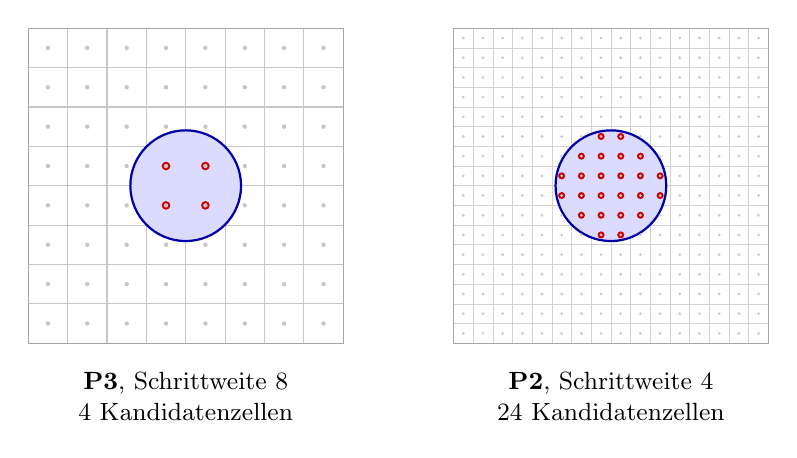
\begin{tikzpicture}[x=1cm,y=1cm]
  % ---------------- P3: Zellen 8 px = 0.5 cm ------------------------------
  \begin{scope}
    \draw[step=0.5,gray!45,thin] (0,0) grid (4,4);
    \draw[gray!70] (0,0) rectangle (4,4);
    \fill[blue!14] (2,2) circle (0.703);
    \draw[blue!65!black,thick] (2,2) circle (0.703);
    \foreach \x in {1.75,2.25}{\foreach \y in {1.75,2.25}{
      \fill[red!80!black] (\x,\y) circle (0.055);}}
    \foreach \x in {0.25,0.75,...,3.8}{\foreach \y in {0.25,0.75,...,3.8}{
      \fill[gray!45] (\x,\y) circle (0.028);}}
    \node[below,align=center,font=\small] at (2,-0.25)
         {\textbf{P3}, Schrittweite 8\\4 Kandidatenzellen};
  \end{scope}
  % ---------------- P2: Zellen 4 px = 0.25 cm -----------------------------
  \begin{scope}[shift={(5.4,0)}]
    \draw[step=0.25,gray!35,very thin] (0,0) grid (4,4);
    \draw[gray!70] (0,0) rectangle (4,4);
    \fill[blue!14] (2,2) circle (0.703);
    \draw[blue!65!black,thick] (2,2) circle (0.703);
    \foreach \x in {1.625,1.875,2.125,2.375}{
      \foreach \y in {1.625,1.875,2.125,2.375}{
        \fill[red!80!black] (\x,\y) circle (0.045);}}
    \foreach \p in {{1.375,1.875},{1.375,2.125},{2.625,1.875},{2.625,2.125},
                    {1.875,1.375},{2.125,1.375},{1.875,2.625},{2.125,2.625}}{
      \fill[red!80!black] (\p) circle (0.045);}
    \foreach \x in {0.125,0.375,...,3.9}{\foreach \y in {0.125,0.375,...,3.9}{
      \fill[gray!40] (\x,\y) circle (0.02);}}
    \node[below,align=center,font=\small] at (2,-0.25)
         {\textbf{P2}, Schrittweite 4\\24 Kandidatenzellen};
  \end{scope}
\end{tikzpicture}
\caption[Kandidatenzellen auf P3 und P2]{Warum ein feineres Gitter hilft.
Dargestellt ist ein Bildbereich von $64\times64$ Pixeln mit einem Objekt von
22,5\px{} Durchmesser -- dem Median des synthetischen Datensatzes. Punkte sind
Gitterzellenzentren, rot markiert sind jene, die in das Objekt fallen und damit
als positive Labelzuweisung in Frage kommen. In der gezeichneten Lage sind es 4
gegen 24; über alle Lagen des Objektzentrums gemittelt 6,2 gegen 24,9
(Tabelle~\ref{tab:p2zellen}). Bei einem ankerfreien Kopf ist diese Zahl das
Trainingssignal, das je Objekt zur Verfügung steht.}
\label{abb:p2zellen}
\end{figure}

Zwei Ablesungen sind entscheidend. Erstens: Für die kleinsten real auftretenden
Objekte steht auf P3 im ungünstigsten Fall nur \emph{eine} Kandidatenzelle zur
Verfügung, auf P2 sind es vier. Ein Objekt, dessen Zuweisung an einer einzigen
Zelle hängt, ist gegenüber der Diskretisierung des Gitters maximal empfindlich --
genau das Problem, das die Small-Target-Aware Label Assignment von YOLO26 auf der
Verlustseite mildert. Zweitens ist der Vorteil \emph{größenabhängig}: Bei
27,4\px{} bietet schon P3 neun Zellen, die zusätzlichen 37 auf P2 ändern wenig.
Die Erwartung lautet also nicht \enquote{P2 hilft}, sondern \enquote{P2 hilft
dort, wo die Objekte klein sind} -- und diese Erwartung ist prüfbar.

\subsection{Ergebnis}

\begin{table}[htbp]
\centering
\caption[Ergebnis des P2-Vergleichs]{Ergebnis des P2-Vergleichs. Oben nativer
Maßstab, unten bei der je Modell nach \mAPall{} auf \code{val} gewählten
Auflösung (\code{yolo26s}: 1600, \code{yolo26s-p2}: 1920); \code{test} blieb an
der Auswahl unbeteiligt. Fett ist je Spalte der bessere Wert.}
\label{tab:p2ergebnis}
\footnotesize
\begin{tabular}{@{}lrrrrrr@{}}
\toprule
\textbf{Modell} & \code{val} \mAPfifty{} &
\code{test} \mAPfifty{} & \code{test} \mAPseven{} & \code{test} \mAPall{} &
\code{test} $F_1$ & \code{test} $P$ / $R$ \\
\midrule
\multicolumn{7}{@{}l}{\itshape nativer Maßstab}\\
\code{yolo26s}    & 0,931 & 0,905 & 0,333 & 0,427 & 0,888 & 0,904 / 0,872 \\
\code{yolo26s-p2} & \textbf{0,936} & \textbf{0,941} &
\textbf{0,387} & \textbf{0,450} & \textbf{0,933} & \textbf{0,975} / \textbf{0,895} \\
\midrule
\multicolumn{7}{@{}l}{\itshape bei der auf \code{val} gewählten \code{imgsz}}\\
\code{yolo26s} (1600)    & 0,939 & 0,905 & -- & 0,427 & 0,888 & 0,904 / 0,872 \\
\code{yolo26s-p2} (1920) & \textbf{0,940} & \textbf{0,947} & -- &
\textbf{0,449} & \textbf{0,934} & \textbf{0,963} / \textbf{0,907} \\
\bottomrule
\end{tabular}
\end{table}

Die theoretische Erwartung bestätigt sich: Bei praktisch identischer
Parameterzahl erreicht \code{yolo26s-p2} auf dem unberührten Testbild
\mAPfifty{} = 0,941 statt 0,905 und \mAPseven{} = 0,387 statt 0,333. Der Gewinn
entsteht dabei \emph{nicht} über die Boxpräzision -- die mittlere Treffer-IoU
sinkt sogar leicht von 0,729 auf 0,728 --, sondern über die Trennung von Objekt
und Hintergrund: Die Precision am Betriebspunkt steigt von 0,904 auf 0,975 bei
ebenfalls höherem Rückruf (0,872 auf 0,895). Das ist mit der Rechnung konsistent:
Ein feineres Gitter senkt die Auflösungsgrenze, an der ein Objekt überhaupt
detektierbar ist; es macht die Boxregression bei 20\px-Objekten aber nicht
genauer. Ein zweiter Befund steckt im Trainingsverlauf: \code{yolo26s} erreichte
sein bestes Modell in Epoche~5 und verbesserte sich danach 20 Epochen nicht mehr,
\code{yolo26s-p2} verbesserte sich bis Epoche~22 -- dasselbe Muster wie im dritten
Befund der Okklusionsablation: Wo mehr nutzbares Trainingssignal je Objekt vorliegt,
sättigt das Modell später.

\subsection{Der Vorteil ist größenabhängig}
\label{sec:p2aufloesung}

Die interessantere Prüfung ist nicht der Vergleich bei einer Auflösung, sondern
das Verhalten über die Auflösung -- denn die Rechnung in
Tabelle~\ref{tab:p2zellen} sagt vorher, \emph{wo} der Vorteil liegen muss.
Abbildung~\ref{abb:p2sweep} trägt beide Sweeps gegeneinander auf.

\begin{figure}[htbp]
\centering
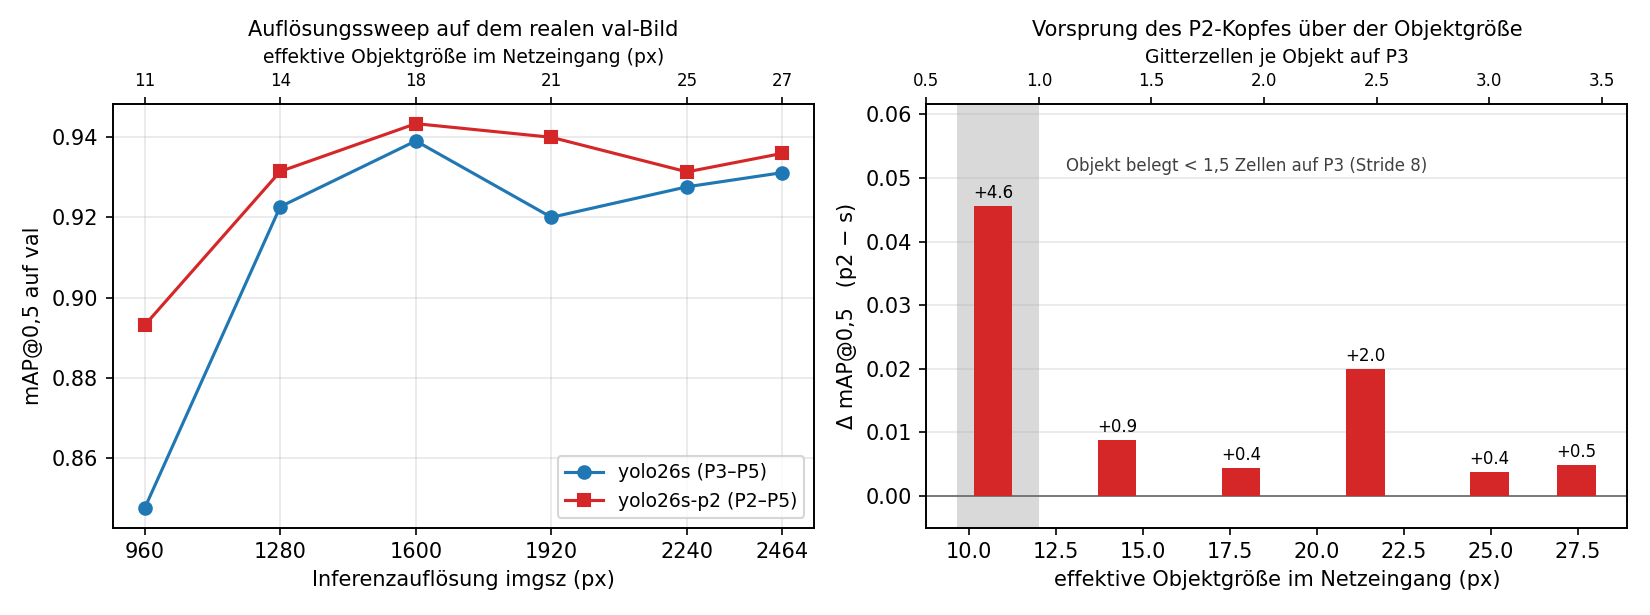
\includegraphics[width=\textwidth]{abbildungen/p2_sweep.png}
\caption[P2-Vorteil über der Auflösung]{Links: \mAPfifty{} auf dem realen
\code{val}-Bild über der Inferenzauflösung für beide Varianten; die obere Achse
nennt die zugehörige effektive Objektgröße im Netzeingang nach
Gleichung~\eqref{eq:deff}. Rechts: die Differenz beider Kurven. Der schattierte
Bereich markiert Objektgrößen unter $1{,}5$ Zellen auf P3, also den Bereich, in
dem die Rechnung aus Tabelle~\ref{tab:p2zellen} den größten Vorteil vorhersagt.}
\label{abb:p2sweep}
\end{figure}

Der Befund entspricht der Vorhersage: Bei \code{imgsz}=960 -- die Objekte
erreichen das Netz dann mit 10,7\px, also 1,3 Zellen auf P3 -- beträgt der
Vorsprung \textbf{4,6\PP}. Er ist damit rund zehnmal so groß wie bei den
Auflösungen, bei denen die Objekte über zwei Zellen belegen (0,4--0,9\PP{} bei
1600 und 1280). Anders formuliert: Der P2-Kopf leistet dasselbe wie eine
Verdopplung der Inferenzauflösung, solange die Objekte klein sind -- und wird
überflüssig, sobald sie groß genug sind. Das ist praktisch verwertbar: Wer die
Aufnahmeauflösung nicht frei wählen kann oder aus Laufzeitgründen bei kleiner
\code{imgsz} inferieren muss, gewinnt durch den P2-Kopf deutlich; wer ohnehin
hochskaliert, kaum. Der Punkt bei \code{imgsz}=1920 fällt mit $+2{,}0$\PP{} aus
diesem Muster; er verletzt die Monotonie und ist -- wie alle Differenzen dieser
Abbildung außer der bei 960 -- vom Konfidenzintervall
(Abschnitt~\ref{sec:bootstrap}) nicht zu unterscheiden.

\subsection{Der Betriebspunkt verschiebt sich stärker als die Detektionsgüte}
\label{sec:p2betriebspunkt}

Ein Nebenbefund des Vergleichs ist praktisch wichtiger als die
Metrikdifferenz selbst und wird leicht übersehen: Das $F_1$-Optimum von
\code{yolo26s-p2} liegt bei $c^* = 0{,}379$, das von \code{yolo26s} bei
$0{,}134$. Der feinere Kopf braucht also eine fast dreifach höhere
Konfidenzschwelle, um seinen besten Betriebspunkt zu erreichen -- er erzeugt
sehr viel mehr Kandidaten mittlerer Konfidenz, was bei $4{,}05$-mal so vielen
Prädiktionspositionen (Tabelle~\ref{tab:p2kennzahlen}) zu erwarten ist. An
diesem Punkt tauscht er Rückruf gegen Precision: 0,975 gegenüber 0,904.

Daraus folgt eine Betriebsregel: Die Konfidenzschwelle des Basismodells darf
\emph{nicht} auf die \code{-p2}-Variante übertragen werden; sie ist je Modell
neu zu kalibrieren, und zwar auf einem Split, der nicht der Testsplit ist --
sonst misst man die Kalibrierung mit. Auf die hier berichteten Zahlen wirkt sich
das nicht aus, weil $c^*$ je Modell aus der Precision-Recall-Kurve bestimmt und
mitberichtet wird.

\subsection{Einschränkungen und Konsequenz}

Drei Vorbehalte sind zu nennen. Erstens beruht der Vergleich auf \emph{je einem}
Trainingslauf pro Variante; die Streuung über Seeds ist unbekannt. Zweitens
liegen alle Differenzen außer der bei \code{imgsz}=960 innerhalb des
Bootstrap-Intervalls. Drittens ist der Vorteil bei \mAPall{} \emph{nicht}
konsistent: Über den Sweep hinweg ist \code{yolo26s-p2} bei drei von sechs
Auflösungen schlechter, was zur unveränderten Treffer-IoU passt -- P2 verbessert
das Finden, nicht das Lokalisieren.

Die Konsequenz für die Arbeit: Der P2-Kopf ist die wirksamste
\emph{architektonische} Maßnahme gegen das in
Abschnitt~\ref{sec:ioukleinobjekt} beschriebene Auflösungsproblem, und er ist
gegenüber der Alternative -- höhere Inferenzauflösung -- die
speichergünstigere Lösung, solange man die Trainingskosten einmalig aufbringen
kann. Für einen produktiven Einsatz wäre \code{yolo26s-p2} zu wählen; die in
dieser Arbeit dokumentierten Experimente~1 und~2 wurden auf der yolo11s-Baseline
gerechnet und bleiben davon unberührt, weil alle drei Modelle auf P3/P4/P5
dieselben Schrittweiten haben.

\fi

\section{Statistische Belastbarkeit und Fehleranalyse}
\label{sec:bootstrap}

Da je Split nur \emph{ein} Bild vorliegt, ist ein gewöhnlicher Bootstrap über
Bilder nicht möglich. Verwendet wird ein räumlicher Block-Bootstrap: Das Bild wird
in Kacheln zerlegt, über die mit Zurücklegen neu gezogen wird (400
Wiederholungen); die Blockbildung ist nötig, weil benachbarte Objekte nicht
unabhängig sind -- sie teilen Beleuchtung, Schärfe und Verdeckungssituation
\parencite{kuensch1989,efron1993}. Für \mAPfifty{} ergibt sich \code{val}
$0{,}892 \pm 0{,}051$ mit 95\,\%-Intervall $[0{,}766;\,0{,}965]$ (23 Kacheln) und
\code{test} $0{,}943 \pm 0{,}023$ mit $[0{,}897;\,0{,}984]$ (25 Kacheln). Alle in
diesem Kapitel berichteten Unterschiede unterhalb dieser Größenordnung sind als
Hinweis und nicht als Nachweis zu lesen; nicht betroffen ist der
Auflösungseffekt, dessen Größe von 47\PP{} das Intervall um ein Vielfaches
übersteigt.

\absatz{Falsch-Negative.} Auf \code{test} sind es am $F_1$-optimalen
Betriebspunkt fünf; sie liegen alle am linken Bildrand und am oberen Stapelrand,
also bei den kleinsten Objekten der Aufnahme. Insgesamt treten sie fast
ausschließlich bei sehr kleinen Objekten, bei stark verdeckten
Enden tief im Stapel -- also dort, wo die Pipeline auch selbst kein Label mehr
vergäbe -- und bei Enden ohne sichtbaren hellen Kranz auf. Letzteres ist der
Fehlertyp, der auf die verbleibende Domänenlücke zurückgeht: Alle vier Clean
Plates sind bei diffusem Licht aufgenommen.

\absatz{Falsch-Positive.} Ihre Ursache unterscheidet sich zwischen den beiden
Bildern, und die Unterscheidung ist nicht kosmetisch. Auf \code{val} haben 9 der
11 Falsch-Positiven \emph{keinerlei} Überlappung mit einer Ground-Truth-Box; ein
Teil von ihnen sitzt auf erkennbaren Rohröffnungen, die in der Annotation fehlen.
Bei 88 handannotierten Objekten schlägt jede fehlende Annotation mit etwa
1,1\PP{} Precision zu Buche, die berichteten Precision-Werte sind also eine
\textbf{Untergrenze}. Die übrigen entstehen an dunklen Löchern im Maschendraht
und an Schattenspalten zwischen Rohren -- genau die Strukturen, gegen die die
Negativbilder gerichtet sind; dass sie dort noch auftreten, spricht dafür, dass
deren Anteil von 9,7\,\% eher an der Untergrenze des Sinnvollen liegt.

Auf \code{test} liegt der Fall völlig anders: Dort tritt am $F_1$-optimalen
Betriebspunkt \textbf{kein einziger Falsch-Positiver} auf, alle 84 Detektionen
sitzen auf annotierten Objekten (Precision 1,000). Der Unterschied liegt in der
Vollständigkeit der Annotation -- auf \code{test} ist jede sichtbare Stirnfläche
erfasst. Die Precision ist dort deshalb exakt und nicht bloß eine Untergrenze.

\section{Ein systematischer Größenversatz der Boxen}
\label{sec:boxversatz}

Der \mAPseven{}-Wert von 0,326 auf \code{test} steht auffällig neben einem
\mAPfifty{} von 0,956: Das Modell \emph{findet} praktisch jedes Objekt, trifft
seine Boxgröße aber systematisch zu klein. Tabelle~\ref{tab:boxversatz}
vergleicht für jede Detektion, die eindeutig auf einem annotierten Objekt sitzt
($\mathrm{IoU} > 0{,}3$), die vorhergesagte mit der annotierten Boxgröße.

\begin{table}[htbp]
\centering
\caption[Größenversatz der Boxen]{Vergleich der vorhergesagten mit der
annotierten Boxgröße. Als Boxgröße dient $\sqrt{\text{Fläche}}$, der
Zentrumsversatz ist in Objektdurchmessern angegeben. \code{sval} ist der
synthetische Split, dessen Labels der Generator selbst erzeugt hat.}
\label{tab:boxversatz}
\footnotesize
\begin{tabular}{@{}lrrrrr@{}}
\toprule
\textbf{Split} & \textbf{Paare} & \textbf{Objekt-\Oe{} (Median)} &
\textbf{pred/GT} & \textbf{GT $-$ pred} & \textbf{Zentrumsversatz} \\
\midrule
\code{test} (real)        &   83 & 20,5\px & 0,888 & $+2{,}29$\px & 0,049\,\Oe \\
\code{val} (real)         &   75 & 27,5\px & 0,961 & $+1{,}16$\px & 0,054\,\Oe \\
\code{sval} (synthetisch) & 1064 & 22,0\px & \textbf{1,012} & $-0{,}29$\px & -- \\
\bottomrule
\end{tabular}
\end{table}

Der Befund ist eindeutig. Auf dem synthetischen Split trifft das Modell die
Boxgröße auf 1\,\% genau; auf den realen Bildern liegt sie 4\,\% (\code{val})
bzw.\ 11\,\% (\code{test}) darunter. Der Versatz ist in \emph{absoluten} Pixeln
annähernd konstant und trifft kleine Objekte deshalb etwas härter: Bei Objekten
unter 18\px{} beträgt das Verhältnis 0,880, bei über 26\px{} dagegen 0,901. Der
Zentrumsversatz liegt mit rund 0,05 Objektdurchmessern (etwa 1\px) im Bereich
der Annotationsgenauigkeit -- es handelt sich also um einen Größen-, nicht um
einen Positionsfehler.

\absatz{Modellfehler oder Labelkonvention?} Weil das Modell auf dem synthetischen
Split die Boxgröße nahezu exakt reproduziert, liegt die Ursache nicht in der
Boxregression, sondern in der \emph{Labelkonvention}: Die Generatorboxen folgen
der $\alpha > 0{,}5$-Kontur der Alphamaske
(Abschnitt~\ref{sec:sichtbarkeit}), die Handannotation umschließt das Objekt
großzügiger. Anforderung~A5 -- identische Labeldefinition in Quelle und Ziel --
ist damit nur \emph{annähernd} erfüllt; der Restversatz beträgt messbar 1,2 bis
2,3\px. Er ist dabei unabhängig von der \emph{Vollständigkeit} der Annotation:
Auf \code{test} ist jedes sichtbare Objekt erfasst -- es gibt dort keinen
einzigen Falsch-Positiven --, und der Versatz tritt trotzdem gerade auf diesem
Split am stärksten auf. Vollständigkeit und Konvention sind zwei getrennte
Eigenschaften eines Labelsatzes.

\absatz{Was der Versatz kostet.} Weitet man alle vorhergesagten Boxen um den
gemessenen medianen Fehlbetrag von 1,15\px{} je Seite auf und wertet neu aus, so
steigt \mAPseven{} auf \code{test} von 0,326 auf \textbf{0,752} und \mAPall{} von
0,466 auf \textbf{0,617}, während \mAPfifty{} von 0,956 auf 0,936 und das $F_1$
von 0,971 auf 0,948 leicht \emph{fallen} (Tabelle~\ref{tab:boxsens} im Anhang).
Die Aufteilung ist damit eindeutig: \mAPseven{} und \mAPall{} auf \code{test}
messen zu einem erheblichen Teil eine Konventionsdifferenz und nicht die
Lokalisierungsgüte des Modells -- sie sind \textbf{pessimistisch}. \mAPfifty{}
und das $F_1$ sind vom Versatz unberührt; dass sie beim Aufweiten sogar leicht
sinken, zeigt, dass an der Zuordnungsschwelle 0,5 nichts mehr zu gewinnen ist.
Es ist \emph{keine} Aussage über ein neu trainiertes Modell, sondern eine
Obergrenzenschätzung für den Effekt einer angeglichenen Labelkonvention.

\absatz{Konsequenz.} Die Korrektur ist einfach und sollte vor jeder weiteren
Optimierung erfolgen: Die Boxen des Generators sind an die Annotationskonvention
anzupassen, indem die Boxschwelle von $\alpha > 0{,}5$ herabgesetzt oder die
fertige Box um etwa 1\px{} je Seite aufgeweitet wird. Sauberer, aber teurer wäre
der umgekehrte Weg -- die Handlabels nach derselben Regel neu zu ziehen, nach der
der Generator seine Boxen bildet. Solange beides nicht geschehen ist, sind die
Lokalisierungsmetriken dieser Arbeit untereinander vergleichbar, nicht aber gegen
Literaturwerte.
